\documentclass[a4paper,12pt,numbers=noenddot]{scrreport}

\usepackage[german]{datetime2}
\usepackage[onehalfspacing]{setspace}
\usepackage[utf8]{inputenc}
\usepackage{amsmath, amsfonts, amssymb, amsthm}
\usepackage{mathrsfs}
\usepackage{graphicx}

\usepackage{scrlayer-scrpage}
\renewcommand*{\chapterpagestyle}{scrheadings}
\clearpairofpagestyles

\ohead{\normalfont \today}
\chead{\normalfont Algebraic Automata Theory}
\ihead{\normalfont \rightmark}

\ofoot{\normalfont Seite~\pagemark}
\cfoot{\normalfont CAU Kiel - Technische Fakultät}
\ifoot{\normalfont Eric Hotho, Klaas Pelzer}

\KOMAoptions{headsepline=true,footsepline=true}
\renewcommand*{\chapterheadstartvskip}{\vspace*{-.4cm}}
\renewcommand*{\chapterheadendvskip}{\vspace{.5cm}}

\setlength{\parindent}{0pt}

\setkomafont{chapter}{\LARGE}
\setkomafont{section}{\Large}
\setkomafont{subsection}{\large}
\setkomafont{subsubsection}{\normalsize}
\setkomafont{paragraph}{\normalsize}
\setkomafont{subparagraph}{\small}
\usepackage[htt]{hyphenat}
\usepackage[german]{babel}
\setcounter{chapter}{2}

\def\lsk{\left<}
\def\rsk{\right>}

\begin{document}
\automark{section}
\automark{chapter}
\chapter{}
\section{}
\section{}
\section{}
\begin{center}
\begin{tabular}{c|cc|l}
x & $q_0$ & $q_1$   \\ \hline
a & $q_0$ & $q_1$   \\
b & $q_1$ & $\bot$  \\
c & $\bot$ & $q_0$  \\ \hline
aa & $q_0$ & $q_1$ & same as a \\ 
ab & $q_1$ & $\bot$ & same as b \\ 
ac & $\bot$ & $q_0$ & same as c \\ 
ba & $q_1$ & $\bot$ & same as b \\ 
bb & $\bot$ & $\bot$ \\ 
bc & $q_0$ & $\bot$ \\ 
ca & $\bot$ & $q_0$ & same as c \\ 
cb & $\bot$ & $q_1$ \\ 
cc & $\bot$ & $\bot$ & same as bb \\ \hline
$\vdots$ & $\vdots$ & $\vdots$ & \\
\end{tabular}
\end{center}
From the table we compute $S(M) = \{[a], [b], [c], [b^2], [bc], [cb]\}$.
Suppose $S(M)$ is a group with $u,v \in \Sigma^*, \delta_u, \delta_v \in \lsk \mathcal{F}(M) \rsk$ then there exists for an arbitrary but fixed $\delta_u$ another $\delta_v$ with $\delta_u \delta_v = id_Q$.
Notice we can choose $q_1\delta_b = \bot$ and we cannot find any $\delta_v$ with $\bot \delta_v = q_1$.
Therefore $S(M)$ is not a group.

Now assume $S(M)$ is a monoid.
Hence, there exists $u \in \Sigma^*, \delta_u \in \lsk \mathcal{F}(M) \rsk$ with $\delta_u = id_Q$.
Notice $\delta_a$ satisfies this condition and acts a neutral element.
Thus, $S(M)$ is a monoid.
\qed

\section{}
We construct the following state machine:
\begin{align*}
    M & = \{Q, \Sigma, \delta\} \\
    Q  & = \{q_{-3}, q_{-2}, q_{-1}, q_0, q_1, q_2, q_3\} \\
    \Sigma & = \{-1, 1\} \\
    \delta(q_i,j) & = 
        \begin{cases}
            q_{i+1},  & \text{for } j = 1 \land q_i \neq q_3\\
            q_{-3},   & \text{for } j = 1 \land q_i = q_{3}\\
            q_{i-1},  & \text{for } j = -1 \land q_i \neq q_{-3}\\
            q_3,      & \text{for } j = -1 \land q_i = q_{-3}\\
        \end{cases}
\end{align*}

\begin{figure}[h]
    \centering
    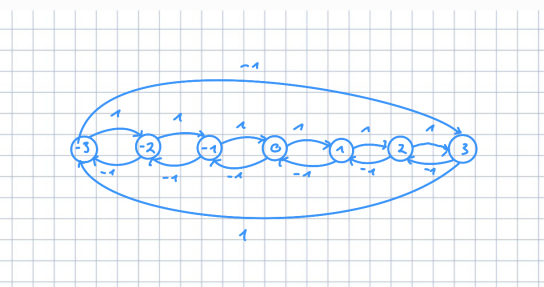
\includegraphics[scale=0.65]{03-automata.png}
\end{figure}

With the following operation table:
\begin{center}
\begin{tabular}{c|ccccccc|l}
    x & $q_{-3}$ & $q_{-2}$ & $q_{-1}$ & $q_{0}$ & $q_{1}$ & $q_{2}$ & $q_3$   \\ \hline
    1-1 & $q_{-3}$ & $q_{-2}$ & $q_{-1}$ & $q_{0}$ & $q_{1}$ & $q_{2}$ & $q_3$   \\ \hline
    1 & $q_{-2}$ & $q_{-1}$ & $q_{0}$ & $q_{1}$ & $q_{2}$ & $q_{3}$ & $q_{-3}$ & shift left  \\ 
    11 & $q_{-1}$ & $q_{0}$ & $q_{1}$ & $q_{2}$ & $q_{3}$ & $q_{-3}$ & $q_{-2}$   \\ 
    111 & $q_{0}$ & $q_{1}$ & $q_{2}$ & $q_{3}$ & $q_{-3}$ & $q_{-2}$ & $q_{-1}$   \\  \hline
    -1 & $q_{3}$ & $q_{-3}$ & $q_{-2}$ & $q_{-1}$ & $q_{0}$ & $q_{1}$ & $q_{2}$  & shift right \\ 
    -1-1 & $q_{2}$ & $q_{3}$ & $q_{-3}$ & $q_{-2}$ & $q_{-1}$ & $q_{0}$ & $q_{1}$   \\ 
    -1-1-1 & $q_{1}$ & $q_{2}$ & $q_{3}$ & $q_{-3}$ & $q_{-2}$ & $q_{-1}$ & $q_{0}$   \\ \hline
    1111 & $q_{1}$ & $q_{2}$ & $q_{3}$ & $q_{-3}$ & $q_{-2}$ & $q_{-1}$ & $q_{0}$ & same as -1-1-1  \\ 
    -1-1-1-1 & $q_{0}$ & $q_{1}$ & $q_{2}$ & $q_{3}$ & $q_{-3}$ & $q_{-2}$ & $q_{-1}$ & same as 111  \\  \hline
$\vdots$ & $\vdots$ & $\vdots$& $\vdots$& $\vdots$& $\vdots$& $\vdots$ & $\vdots$ & \\
\end{tabular}
\end{center}

This gives us $S(M) = \{[-1-1-1], [-1-1], [-1], [1-1], [1], [11], [111]\}$.
With the following isomorphismus $f$ we can map each equivalence class $[w]$ with $w \in \Sigma^*$ to an item of $\mathbb{Z}_3$:
\begin{align*}
    f([w]) = 
    \begin{cases}
        ((|\sum_{u \in w}(u)| + 3) \text{ mod } 7) - 3 & \text{ for } \sum_{u \in w}(u) \geq 0 \\
        -((|\sum_{u \in w}(u)| + 3) \text{ mod } 7) - 3 & \text{ for } \sum_{u \in w}(u) < 0 \\
    \end{cases}
\end{align*}
Here we sum up all right and left shift operations resulting in an all in all right or left shift (or no shift if 0).
If we shift more than 3 in one direction,  we switch back to shifting in the other direction, i.e. $\delta_{1111} = \delta_{-1-1-1}$.

\begin{center}
\begin{tabular}{c|c}
    $[w]$ &  $\mathbb{Z}_3$ \\ \hline
    $[-1-1-1]$ & -3\\ 
    $[-1-1]$ & -2\\ 
    $[-1]$ & -1\\ 
    $[1-1]$ & 0\\ 
    $[1]$ & 1\\ 
    $[11]$ & 2\\ 
    $[111]$ & 3\\ 
\end{tabular}
\end{center}
\end{document}
